
\chapter{指数分布を使った統計モデル}
あるシステムの故障発生間隔日数を調べてみると、次のようなデータを得たとする(実際には、平均10の指数分布関数を使いサンプリングを行った。もちろんそんなことは忘れて、現象は数学関数により生成されていないと考える)
\begin{lstlisting}
19.9290003   0.60892905  0.55864947 29.77846887  0.28955969  1.58223429 21.10080586 10.78952122  0.59624638 15.74379646
\end{lstlisting}


平均値は10.09,分散は107.7であった。以下の仮定からなる統計モデルを構築した。
\begin{quote}
    \begin{enumerate}[(1)]
\item i.i.d
\item 正規分布
\item 平均10.09、分散107.7
\end{enumerate}
\end{quote}
では統計量を元に、$p$値を求めてみる。具体的には、

\begin{lstlisting}
Y =[19.9290003 ,  0.60892905,  0.55864947, 29.77846887,  0.28955969,  1.58223429, 21.10080586, 10.78952122,  0.59624638, 15.74379646]
stats.ttest_1samp(Y, 10.09)
\end{lstlisting}

結果、$p=0.978$である。$p=0.05$を基準にすれば、この統計モデルは棄却できない。統計モデルの仮定が妥当かを一つずつ調べる。統計モデルの仮定(2)は、分布が正規分布であることを仮定している。実際の標本をQ-Qプロットしてみよう。正規分布だと考えても問題がなさそうである。統計モデルの仮定(3)について検討する。このサンプルの平均値は$10.09$なので、これについても仮定は妥当だと考えられる。
では、帰無仮説を採択し、この統計モデルを元に推測をするべきだろうか。このモデルで推測を行なってみる。$15$日後の故障発生率は$P(X>20)=0.0036$程度である。同様に、$5$日後の故障発生率は、$P(X>5)=0.0036$である。正規分布は左右対称な関数なので、平均故障発生日から5日でも15日でも、同じ割合で故障する。 
機械などの故障は日数がたてば故障しやすくなるので、肌感覚としてあり得ないと思われる。
実際に、この統計モデルによる故障発生間隔の推測は現実と乖離していくことがわかっている。
このように、恣意的に決めた$p$より大きな統計モデルを使ったとしても、推測がうまくいくわけではないことから、棄却されなかった統計モデルを採用することには慎重になるべきである。

二つ目は、データの偏りによって、統計モデルを棄却できないことあるということである。
$10000$回実験を繰り返したとして(もちろん、指数分ぷからサンプリングを行った。もちろんそんなことは忘れて、現象は数学関数により生成されていないと考えてください)、サンプルサイズは毎回10だとすると、棄却できる割合は0程度であった。一方で、サンプルサイズを$100$程度にすると、棄却できる割合は、$0.956$程度であった。これは、平均値のあたりにデータが集まりやすく、データの端は無視できる程度の数量しか発生しないことで、正規分布を使った統計モデルを棄却しにくくなる。TODO
このように、データが十分ない場合は$p$の棄却に正規分布を仮定した統計モデルでは統計モデルを棄却する頻度は高くなることが予想される。

$p$値による判断がうまくいかないことがわかった。また、信頼区間の中にある母数でも推論ができないこともわかった。
\if 0
このような偏ったデータを手に入れた場合はどのように統計モデルを作ればいいのだろうか。
\fi

https://biolab.sakura.ne.jp/small-sample-t-test-glm.html



\subsubsection{モデルの更新}
\if 0
データ数の問題と、推測の精度の問題を解決することはできるだろうか?
尤度ひ検定
\fi
月日は流れ、データが蓄積された。その結果、次のような分布が得られた。ここまでの議論で、正規分布を仮定したモデルを棄却できないことはわかった。では、そのモデルを使って現在のデータを予測できるだろうか?パラメータを推定した正規分布とデータの分布を見てみよう。
データの最頻値が0の近くなので、平均10の正規分布では、ズレが生じることがわかる。
これではデータを捉えることはできない。
また、$30$日後までに故障が発生する確率を計算してみると、$0.971$程度であり、30よりも大きなデータの数は$0.05(1-0.05=0.95)$それなりに良く一致している。
一方で,5日までの故障発生率は、$0.30$をと予測するが、実際のデータは、0.18程度であり、こちらは乖離していると感じるだろう。
\begin{figure}
\begin{center}
    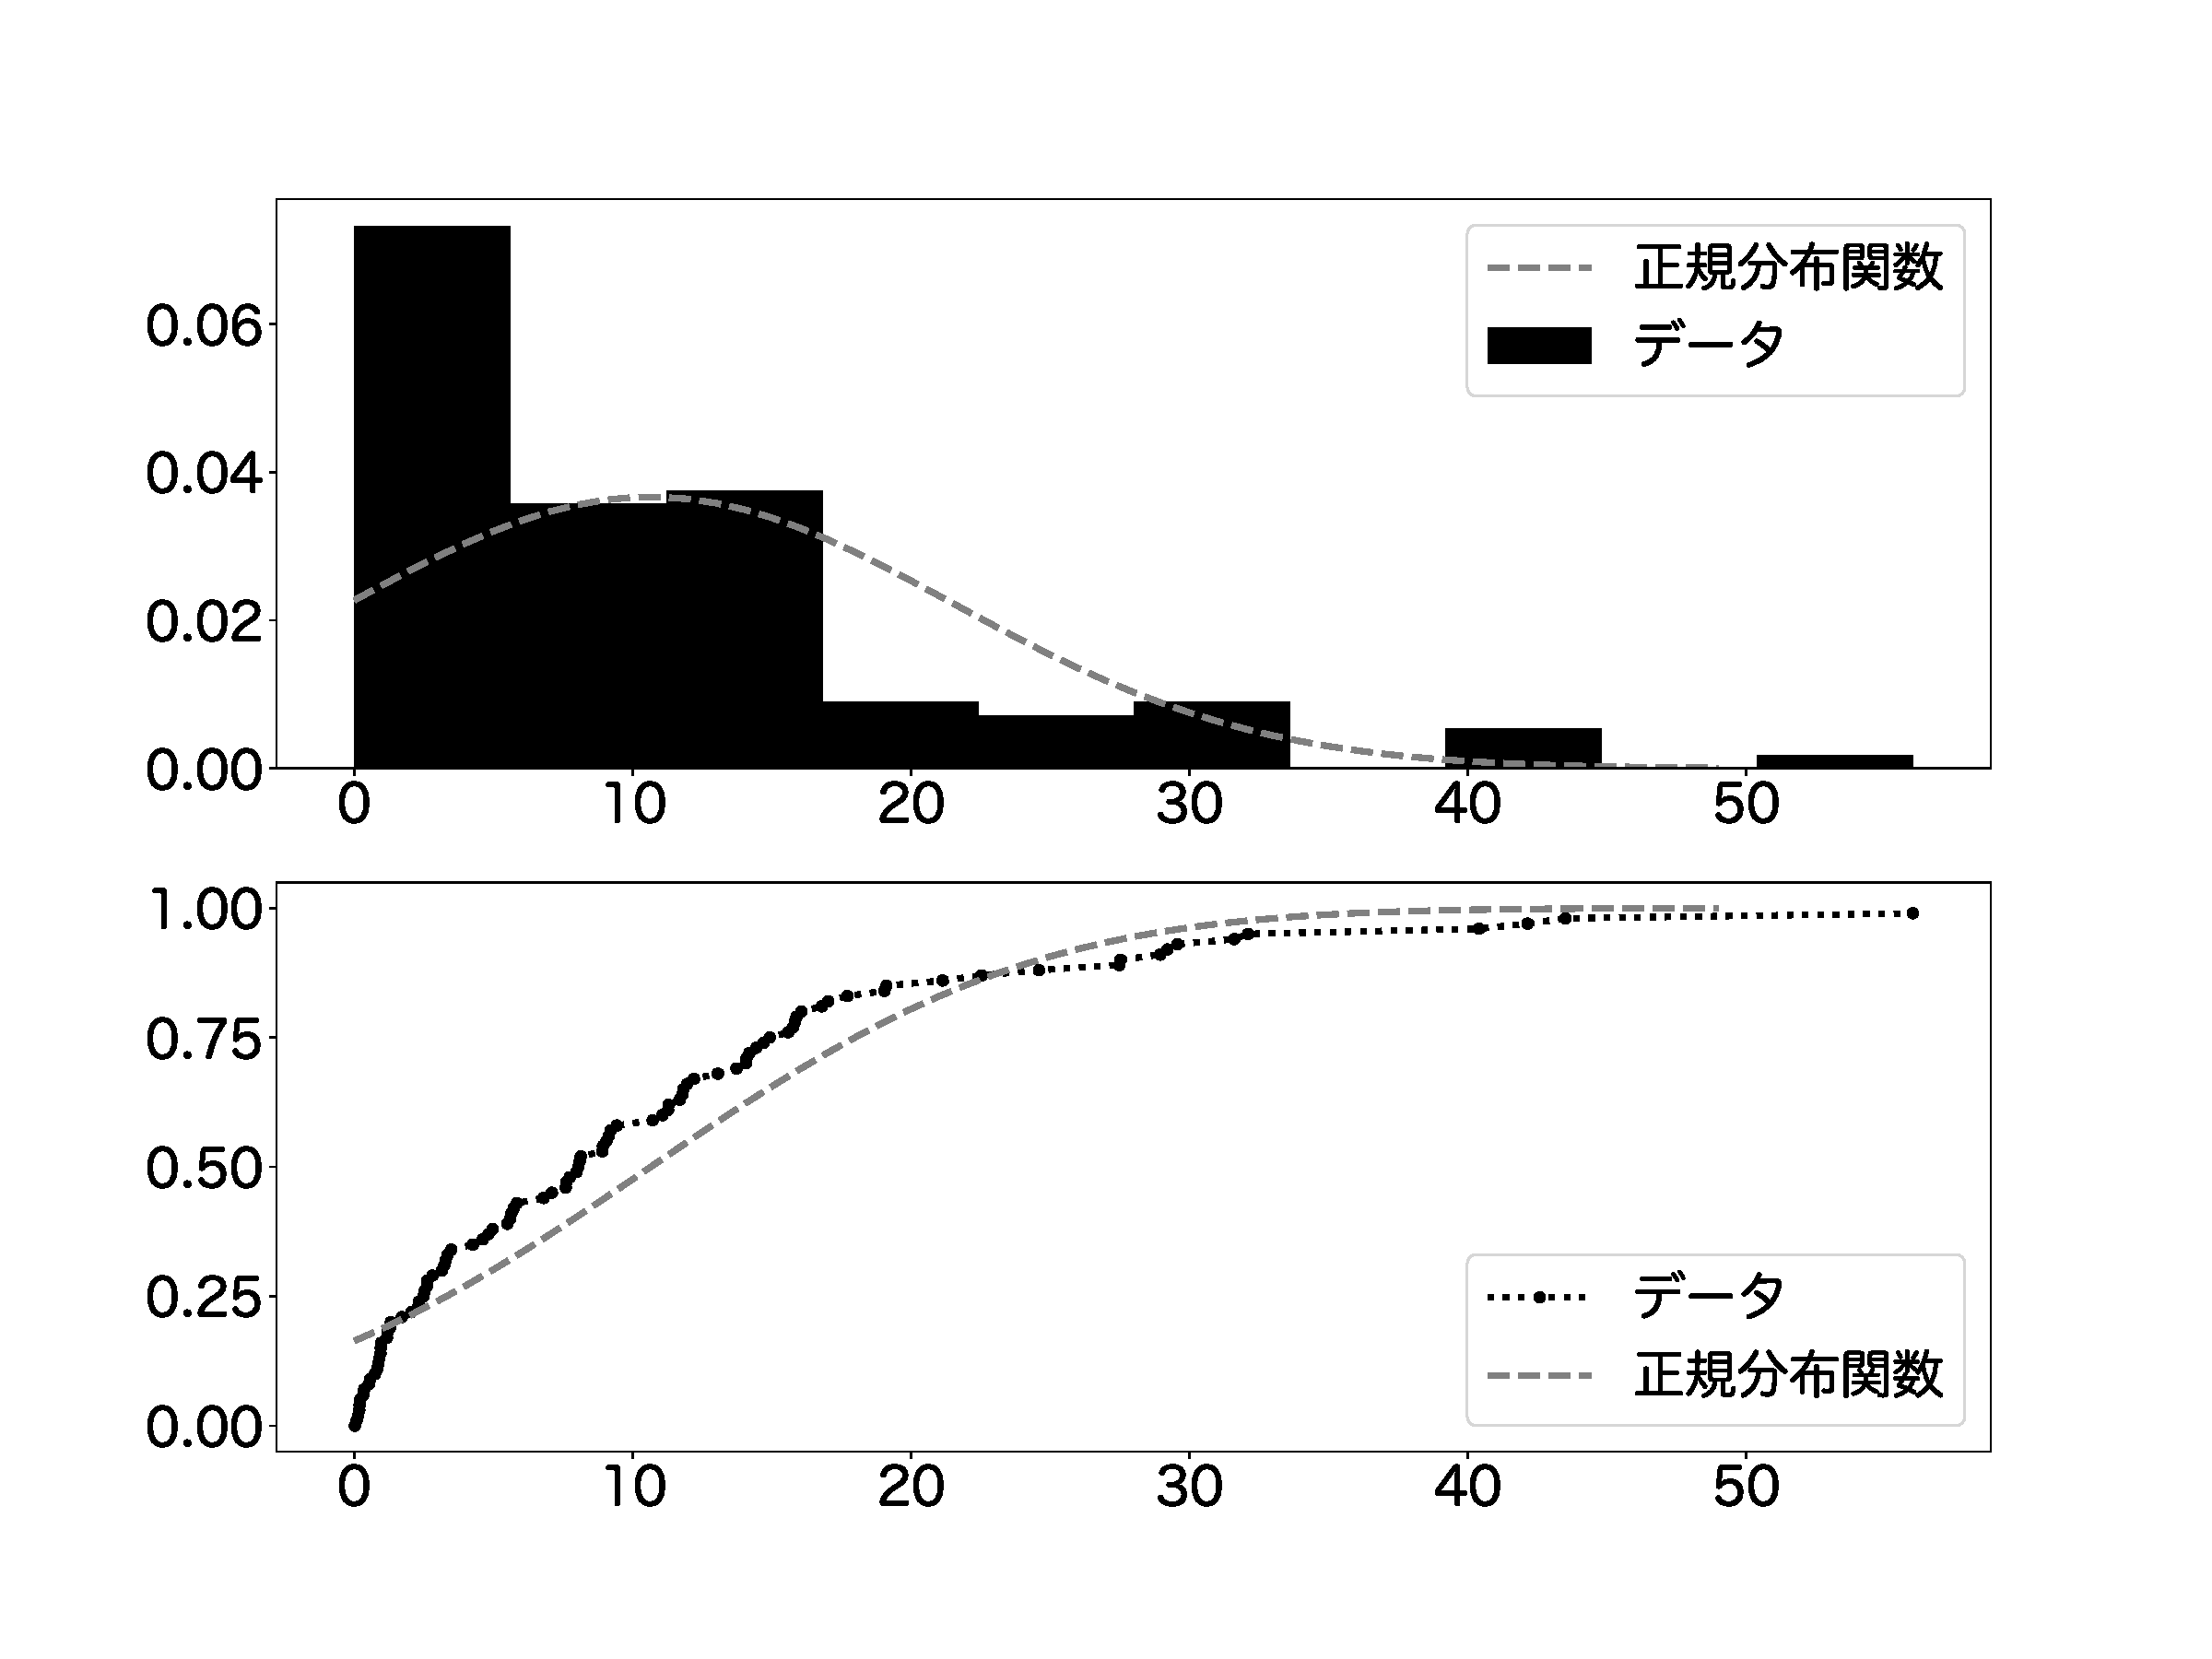
\includegraphics[width=15cm]{./image/06_/normal_exponential.pdf}
    %\caption{データの分布を正規分布で捉えれない}
\end{center}
\end{figure}


では、どのようなモデルを構築すればいいのだろうか。指数分布関数を使ってみよう
\begin{quote}
    \begin{enumerate}[(1)]
\item i.i.d
\item 指数分布
\item 母数$\lambda$
\end{enumerate}
\end{quote}
このモデルを$M(\lambda)$とかく。指数分布では、確率変数の平均は、母数$\lambda$の逆数であることがわかっている($E[x]=\frac{1}{\lambda}$)。$\lambda$として、現在手に入れたデータの平均値の逆数を代入し、データの分布と指数関数の曲線を書いてみると、よく一致しているように見える。

30日後に故障が起こる可能性は、$0.94$程度であると予想が出る。現状のデータと確認をしてみると、30よりも大きなデータの数は$0.05(1-0.05=0.95)$より、良く一致していることもわかる。
\begin{figure}
\begin{center}
    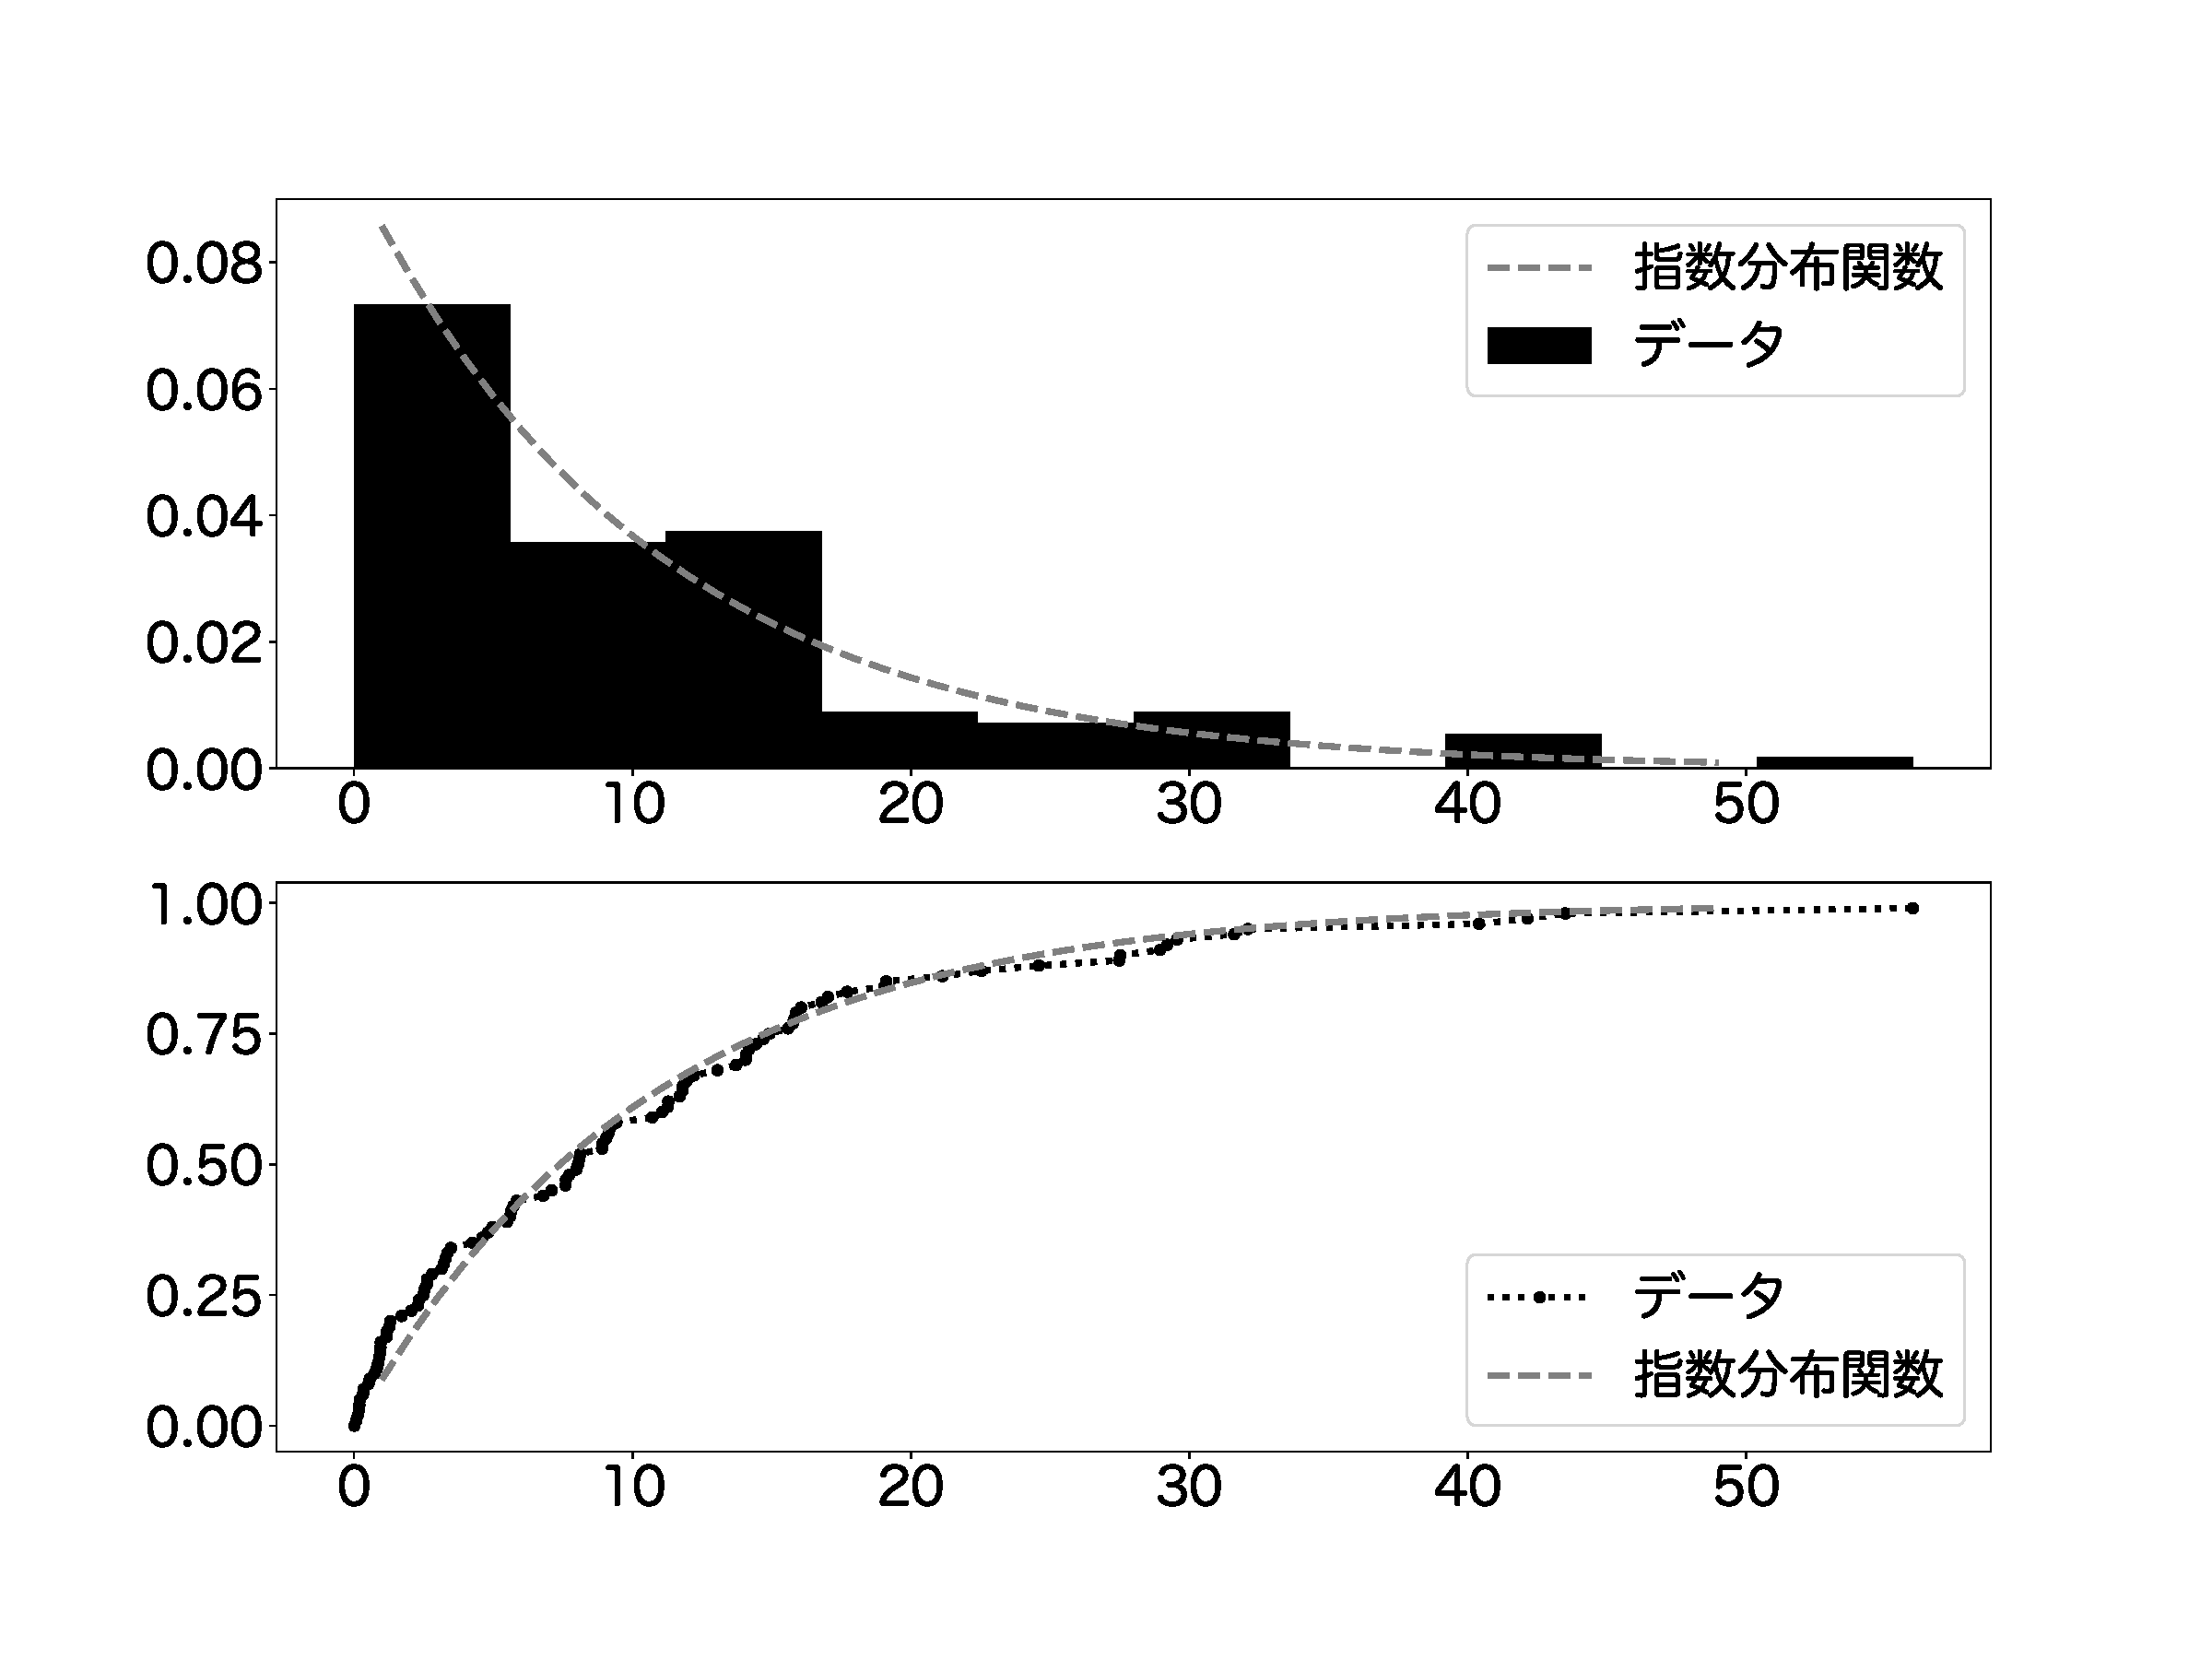
\includegraphics[width=15cm]{./image/06_/lambda_0.1.pdf}
    %\caption{しばらくした後の故障頻度の分布図}
\end{center}
\end{figure}





以上を通じて、単純に正規分布を仮定したモデルを導入すれば良し!とは言えないことがわかっただろう。言い換えれば、サンプルサイズが増えたときに見えてくる分布関数から母集団の構造を想定し、統計モデルを構築するべきだという方針が理解できる。
また、データの構造を理解した上で、推測を行うことで、データと推測が程よく一致することがわかった。


% https://biolab.sakura.ne.jp/small-sample-t-test-glm.html
\if 0
AICでモデルを選ぶと、正規分布の仮定がある。指数関数に対しては選択できないのでは? 
\fi
% https://eprints.lib.hokudai.ac.jp/dspace/bitstream/2115/49477/6/kubostat2008e.pdf
% http://www.ieice-hbkb.org/files/01/01gun_12hen_01.pdf




\paragraph{AAA}
あるとき、「改良することで故障日が伸びたみたいなんだ。調査してくれ」と依頼された。サンプルサイズは10程度であり、以下のようになった(今回も指数分布を使ってデータを生成した。もちろん実際の現象は数学の関数で生成されているわけではない)。

\begin{lstlisting}
6.46239039  7.5235678  31.84227772  6.73334029  2.9221049   1.84776618  8.7189158   2.97501827 57.78271493 20.51976339
\end{lstlisting}

統計モデルを構築しよう。
\begin{quote}
    \begin{enumerate}[(1)]
\item i.i.d
\item 正規分布
\item $\mu=10$
\end{enumerate}
\end{quote}

とする。以前のデータ解析では、指数関数を利用し、その平均値は10程度であった。今回の統計モデルでは平均$10$の正規分布を利用することで、この統計モデルが棄却できるかを試してみよう。



\begin{lstlisting}
stats.ttest_1samp(Y, 10)
\end{lstlisting}




その結果、$p=0.421$であることがわかった。このことから、有意水準$p<0.05$を満たしていないので、帰無仮説は棄却で聞いないので、改良できていないという判断を行うべきだろうか?
もちろん良くない。モデルの仮定をみると、統計モデルの仮定(2)が正規分布になっている。これは、我々が扱っている標本にはうまく適応できないことが経験的に理解してきた。
では、次のモデルはどうでしょう。

\begin{quote}
    \begin{enumerate}[(1)]
\item i.i.d
\item 指数分布
\item 指数分布の母数$\lambda=0.1$
\end{enumerate}
\end{quote}
このモデルは、故障日をよく予測してくれることがわかっている。
今回、統計モデルが正規分布ではないので、これまでの仮説検定により、統計モデルとデータの乖離を評価できない。そこで、数理統計学の知識を使う。

\subsection{指数分布関数の仮説検定}
確率変数$X_1,X_2,\cdots,X_n \sim i.i.d \ Exp(\lambda)$は、$n\bar{X}\sim Ga(1,\frac{1}{\lambda}) $ただし、$\bar{X}=X_1+X_2 \cdots +X_n$ここで、$Ga(1,\lambda)$は、尺度母数$\lambda$のガンマ分布である。統計量$\bar{X}$を利用した検定ができることが示唆される。
%https://ds.machijun.net/clear-exercise-of-statistics/%E7%AC%AC7%E7%AB%A0-%E6%8C%87%E6%95%B0%E6%AF%8D%E9%9B%86%E5%9B%A3ex%CE%BC%EF%BC%89%E3%81%AE%E6%AF%8D%E5%B9%B3%E5%9D%87%E3%81%AE%E4%BF%A1%E9%A0%BC%E5%8C%BA%E9%96%93%E3%81%A8%E6%A4%9C%E5%AE%9Ap128/



\subsection{尤度比検定}
TODO: 尤度比検定の定義

我々のデータをもとに推論をすると、
$$
\eta= \frac{\lambda_0\exp\left({-\lambda_0\sum x_i}\right)}{\bar{\lambda}^n \exp{(-n)}}
$$
ここで、$\bar{\lambda}$は最尤推定量であり、$\frac{n}{\sum x_i}$、$\lambda_0=0.1$,$n$はサンプルサイズである。
以上を元に、$\eta$を計算する。
$$
-2\log \eta \sim \chi^2_1
$$

より、$p=0.1902$と計算できる。$p$値を計算したら、やることはいつも同じで、統計モデルの仮定をもう一度調べる。統計モデルの仮定(1)はおそらく問題ない。統計モデルの仮定(2)は、少しの改良を加えただけなので、母集団の特性はほとんど変わっていなと前提を置いているので、悪くない近似ができることを期待している。統計モデルの仮定(3)は、$\lambda=0.1$である。$p>0.05$より現状では母数$\lambda$が変化しているとは言い切れない。




\begin{lstlisting}
9.70693386 14.74490149 33.03244855 21.8343649  40.73749837
\end{lstlisting}


さらにサンプルサイズが増えた。この場合、$p=0.01325$となり、$p=0.05$の有意水準を満たす。$N$数をどこまで増やすべきだったのだろうか。

TODO いつかかくけど、どこまで増やすんだろうか。
理想的には構造がわかるまで計測できたら嬉しい



\subsection{分散分析}
Section.2で行った分析では、様々な母平均に対して、統計モデルの推定がデータと一致することを確かめた。今回は、ばらつきを変化させ、統計モデルと推定の一致について考えてみよう。
統計モデルを構築しよう。
\begin{quote}
    \begin{enumerate}[(1)]
\item i.i.d
\item 正規分布$N(170,\sigma^2)$
\item 正規分布の母数$\sigma$
\end{enumerate}
\end{quote}
このモデルを、$M(\sigma)$とする。身長を予測するモデルとして、分散を替えてみよう。
Section.2で利用していた$M(5.7)$に対して、$M(10.0)$が現象を推定可能かを検討してみよう。
分布関数を書いてみると、グラフの裾野が広がったことが見て取れる。その分、ピークである$170$のあたりの頻度が減少している。つまり、$170$が出てくる頻度が下がり、より様々な身長の人がサンプリングできることが期待される。一方で、$M(2.0)$では、$170$の辺りが増え、他の場所では、頻度が現象することがわかる。$M(5.7)$よりも、身長のバラエティが少ないデータにたいし適合できる。


\begin{lstlisting}
163.54258776 179.15834405 172.6934295  166.29185695 177.65182141 165.87491547 172.08610141 158.30711988 163.74574501 176.47887419
\end{lstlisting}




拒否するべき統計モデルはどのような母数をもつだろうか。
10人から無作為抽出したデータに対して、統計モデル$M(3.1),M(12.0)$は十分データを説明できるだろうか?
統計モデルの上で、確率変数$X_1,X_2,\cdots,X_n$から計量される以下の統計量を定義する。
$$
Y_0=(n-1)\left(\frac{S_x}{\sigma}\right)^2
$$
ここで、$S_x^2=\frac{1}{n-1}\sum_{i=0}^{n}(x_i-\bar{x})^2,\bar{x}=\frac{1}{n}\sum_{i=0}^{n}x_i$である。
統計量$Y_0$は、$Y_0\sim\chi^2_{n-1}$であることがわかっている(定理\ref{fig:normal_sigma_chi2})。
このとき、$M(3.1),M(12.0)$については、$p<0.05$となり棄却される。
$p$値を基準にして、絶対にだめな統計モデル$M(3.1)$から、サンプリングを行ってみる。
\begin{lstlisting}

165.02227239, 163.16327065, 170.40109545, 170.81675656, 167.80872784, 166.91030856, 167.24096441, 170.44877048, 165.99400494, 167.59131488
\end{lstlisting}

統計モデル$M(5.7)$よりも値が広がった印象があると直ちにはわからない。
$M(3.1)$を使って、$180cm$を超える人の割合を計算すると、$P(X>180)<10^-5$となり、観測と比較してかなり少ない。
同様に、統計モデル$M(12.0)$を使って計算を行うと、$P(X>180)=0.15$となり、観測と比べて多いこともわかる。
棄却されなかった統計モデル$3.1<\sigma<12.0$の中でも、積極的に予測に利用するには、データの構造をより理解する必要がある。


\begin{figure}
\begin{center}
    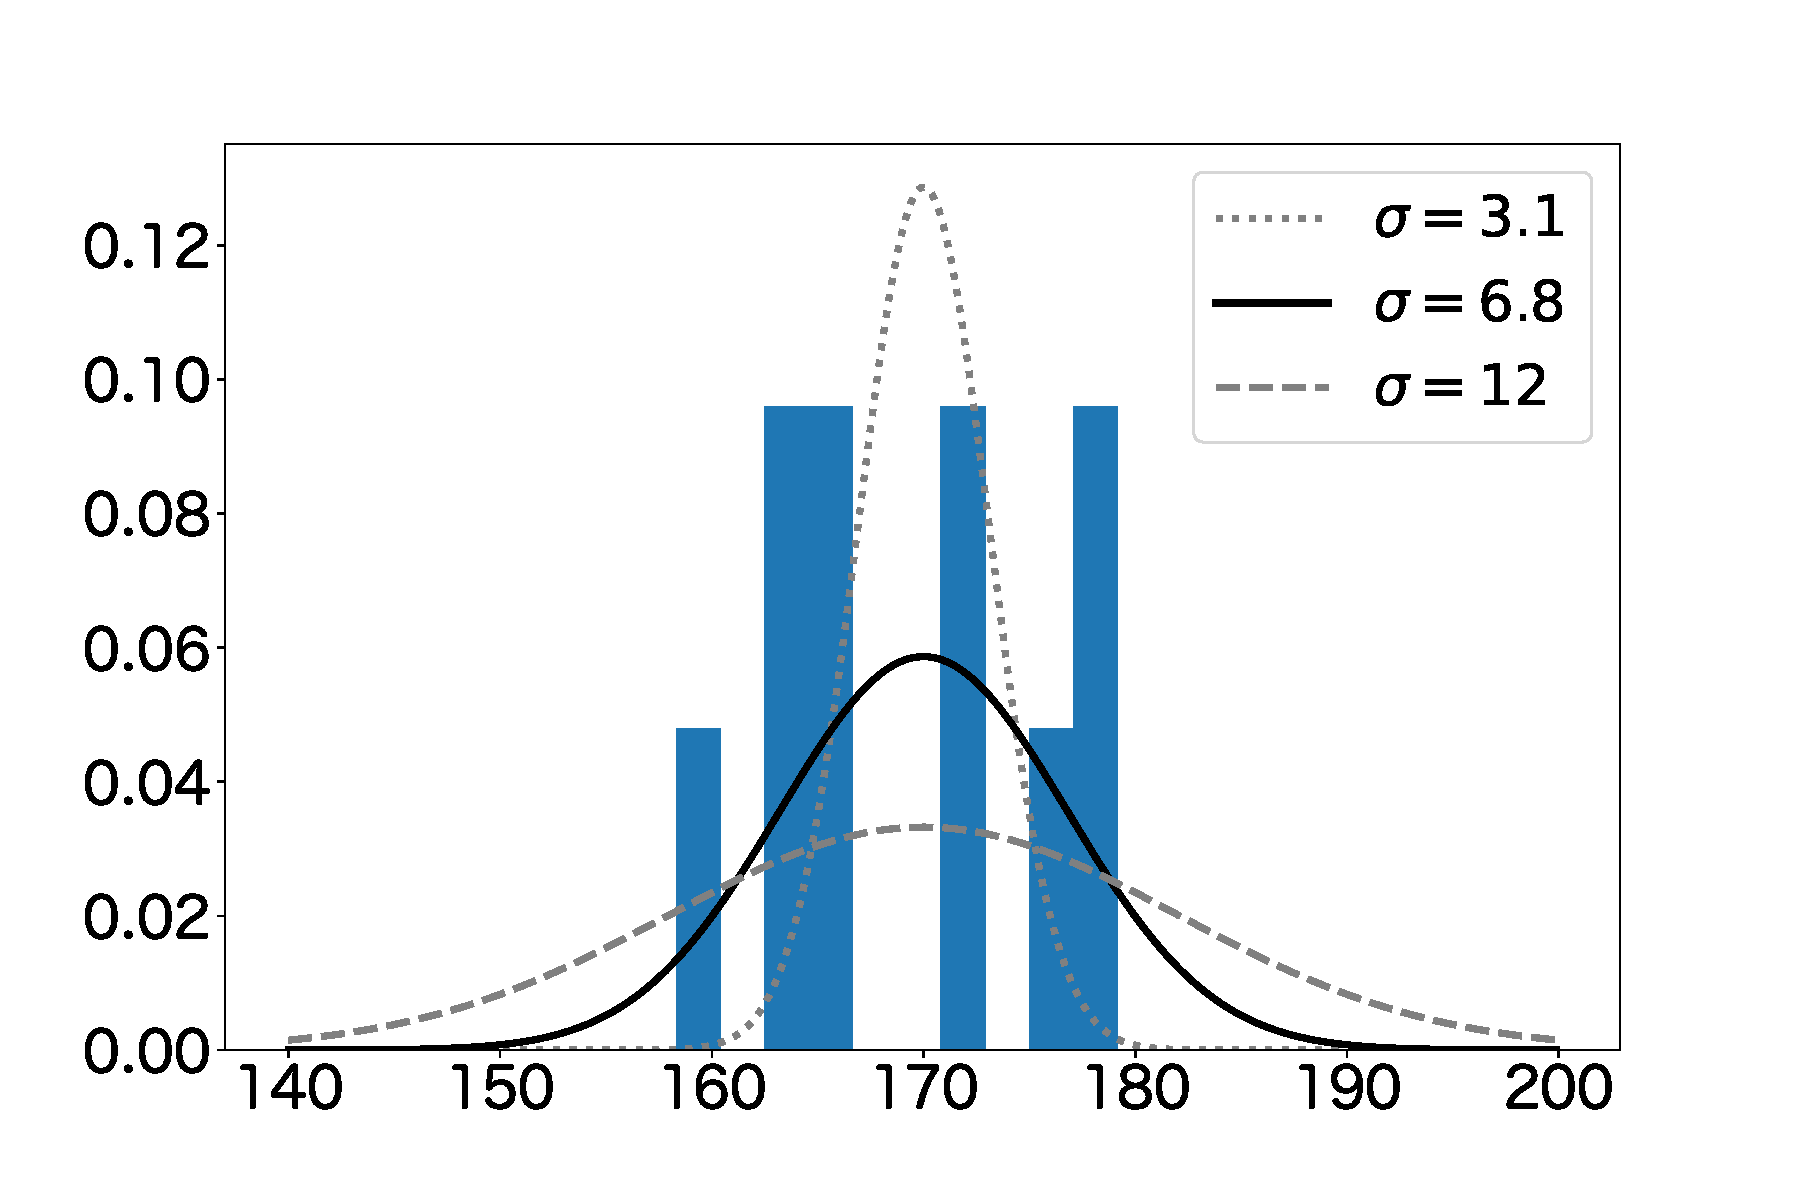
\includegraphics[width=15cm]{./image/06_/normal_sigma.pdf}
    %\caption{検出力}
\end{center}
\end{figure}

\if 0
https://biolab.sakura.ne.jp/welch-test.html
https://biolab.sakura.ne.jp/welch-anova-statwing.html
https://biolab.sakura.ne.jp/welch-test.html
\fi

